\newpage
\section{\ac{SVAR} Identification} \label{SVARIdentification}

For implementaiton of the methods introduced in previous section the SVAR package in R \footcite[See.][]{Lange2020} software is used.
\subsubsection{SVAR Model Identification}
The structural VAR models are often used to trace the contemporaneous linkage among macroeconomic variables. The SVAR model has the following general form  \footcite[Source: See][]{Lange2020}: 
\[ A_0 Y_t = mu+  A_1(L) Y_t + B \epsilon_t \]
where yt = [y1t
, ..., yKt]
 is a vector of observable variables, Ai
, i = 1, . . . , p, are (K × K)
coefficient matrices, and intercept parameters are collected in µ. We focus on the case of time
invariant deterministic terms for notational clarity. Model augmentation with time-varying
deterministic terms (e.g., breaks, linear trends), however, is straightforward. Furthermore,
the VAR model is stationary (invertible) by assumption. The vector ut consists of reducedform residuals, which are serially uncorrelated with E(ut) = 0 and Cov(ut) = sigmau. The
nonsingular matrix B captures the instantaneous effects of the structural shocks
on the variables of the system
 Where $Y_t$ is n-vector relevant variables, then $A_0$ and $B$ are $n * n$ matrices and $A_1(L) = \sum\limits_{i=1}^ qA_{1i} L^i $ is the matrices polynomial in the lag operator in which $A$ matrices have the same size as $A_0$ matrix. The error terms$\epsilon_t$ (structural schocks) is an n-vector of serially uncorrelated zero mean structural schocks with and identitiy contemporanous covariance matrix. The crucial part in SVAR modelling is the choice of the macroeconomics variables. The second challenge is that the nmuber of parameters to be identified in the structural model is larger than that of the reduced VAR form. Therefore, some new relations needs to be introduced. This can be usually done by introducing restrictions on $A_0$ or $B_0$ matrix. 

In this work, we assume the following set of variables as the variables involed in modeling. 
The assumed $Y$ is :
\[ 
 \begin{bmatrix}
        ry \\ 
        \pi \\
        rg \\
        r \\
        mc \\
        h \\
        hp \\
  \end{bmatrix}
\]

r is the money market interest rate (EONIA) rate at which banks provide loans to each other with a duration of 1 day, In my opinion this is a good indicator of the monetary policy since it combines central banks ECB's deposit facility rate and  s. This affect is more clear when we look in the recent data after 2018 where central banks interest rate for refinancing is zero but the deposit facility goes negative and this stimulates banks to lend more money. Original data is monthly and we need to average to get the yearly rate. See https://www.bundesbank.de/en/statistics/time-series-databases

rg is
General government deficit(-) or surplus(+) as defined in the Maastricht Treaty from  Bundes Bank is used, In my opinion it is a good indicator of the Government fiscal policy since it includes both expenditure and earinging of the gorvernment. Change in percentage for each year is calculated and sign is reversed such that when the governemnt has a deficit it is an indicator if positive government spending.

ry is
Germany / National accounts / Overall economy / Gross domestic product (price adjusted) 1, 2, 3

hp is 
Real house prices, 2015=100, adjusted! https://data.oecd.org/price/housing-prices.htm
cite: OECD (2020), Housing prices (indicator). doi: 10.1787/63008438-en (Accessed on 18 May 2020)
mc 
change in percent Construction price index / Germany / Unadjusted figure / Total  bundes bank

h
west germany is used as trend is the same in east! this is the only free source of data I could find for this period.
 https://www.statista.com/statistics/999254/number-completed-new-dwellings-west-germany/ in thousenad

The variables are chosen based on the model proposed in housing in Australia \footcite[See.][]{Wadud2009} based on supply and demand model with a modification that the exchange rate and foreign interest rates are ommited from demand equation. The resulting equatioins are as follows:

\[ 
h^s = a_1 mc + a_2 rhp + b_1^s \epsilon^s
h^d = a_3 ry + a_4 rhp + a_5 r + a_6 /pi + a_7 rg  + b_1^d \epsilon^d
h^s = h^d
\]
The notion of time is deleted from the above equation but once can consider that the every variable reperesnt different time instance for example $a-1 mc$ depending on the cohsen number of lags represent $a_{1t} mc_{t} ,  a_{1(t-1)} mc_{(t-1)} ...  $
this will lead to 
\[
 rhp  = c_1 mc+  c_2 ry + c_3 rhp  + c_4 r + c_5 /pi + c_6 rg  + b_1 \epsilon
\]

The second assumption chosen by author in this work is that $A_0$ is a lower triangular matrix therefore as one can see in the order of variables in bla equation every variable can have only correlation with previous variables in the same time stamp and with all variable in previous time stamps. Therefore, the order of variables play a crucial role in our model. 


\subsection{SVAR Results}
The following picture shows the results of the identified model to different schocks
\begin{figure}[H]
\caption{Interest Rate, Government Spending and House Price in Germany in Years 2000-2020}
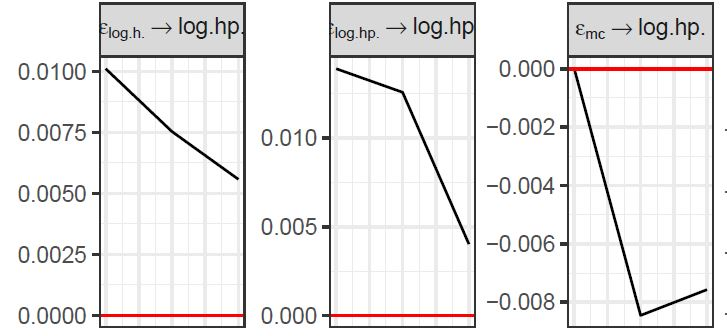
\includegraphics[width=0.9\textwidth]{hp1}
\\
\cite[Quelle: Own Graph][]{FOM}
\end{figure}
\begin{figure}[H]
\caption{Interest Rate, Government Spending and House Price in Germany in Years 2000-2020}
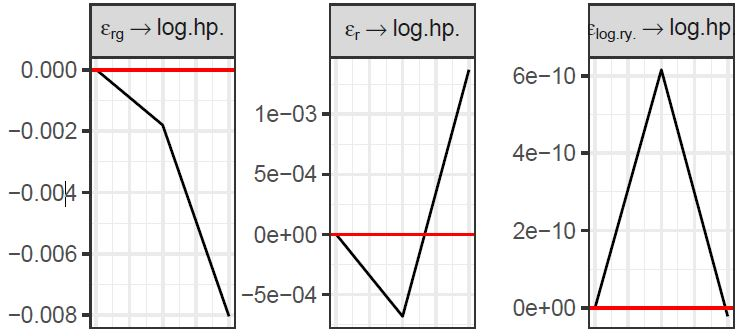
\includegraphics[width=0.9\textwidth]{hp2}
\\
\cite[Quelle: Own Graph][]{FOM}
\end{figure}


